\documentclass[norsk]{beamer}
 
\usepackage[T1]{fontenc}
\usepackage{textcomp,pdfpages}
\usepackage{babel}

\usepackage{amsmath, amsfonts, epsfig, xspace}
\usepackage{pstricks,pst-node}
\usepackage{multimedia}
\usepackage{beamerthemesplit}
\usepackage[absolute, overlay]{textpos}

\usetheme{bekk}


\author{Aslak Johannessen \\ aslakjo@bekk.no  @aslakjo}

\title[Scala kurs]{Fagkveld hos BEKK -- Scala}
\subtitle[]{Introduksjon til scala}
\institute{BEKK Consulting AS}


\begin{document}

\maketitle

\begin{frame}{Velkommen}
  \begin{content}
    \begin{itemize}
  		\item Hvorfor scala?
	  	\item Kurs
		  	\subitem{Litt foiler}
         	  	\subitem{Litt oppgaver}
	  	\item Middag
	\end{itemize}
  \end{content}
\end{frame}

\begin{frame}{Oss}
Rune
Eivind
Ole Christian
Torbj�rn
Kai
Stein K�re
Aslak
\end{frame}

\kontrast{Hvorfor scala?}

\kontrast{Hvorfor scala?\small\\\hfill\\Java er gammelt\\Scala er et riktig steg videre\\Bedre konsepter $\equiv$ bedre kode}

\begin{frame}[containsverbatim]{Gammelt}
 \begin{content}
    \begin{lstlisting}[basicstyle={\tiny\ttfamily}]	   
public class Person{
    private String navn;
    private String etternavn;
    private Integer alder;

    public Person(String fornavn, String etternavn, Integer alder){
        this.navn = fornavn;
        this.etternavn = etternavn;
        this.alder = alder;
    }

    public String fulltNavn(){
        return navn + " " + etternavn;
    }

    public String getNavn(){ return navn; }
    public void setNavn(String navn){ this.navn = navn; }

    public String getEtternavn(){ return etternavn; }
    public void setEtternavn(String etternavn){ this.etternavn = etternavn; }

    public Integer getAlder(){ return alder; }
    public void setAlder(Integer alder){ this.alder = alder; }
}
     \end{lstlisting}
  \end {content}
\end{frame}

\begin{frame}[containsverbatim]{Nytt}
 \begin{content}
    \begin{lstlisting}[basicstyle={\small\ttfamily}]	   
class Person(
  val navn:String, 
  val etternavn:String, 
  val alder:Int)
{
  def fulltNavn ={
    "%s %s".format(navn, etternavn) 
  }
}
     \end{lstlisting}
  \end {content}
\end{frame}

\kontrast{Closure}


\begin{frame}[containsverbatim]{Gammelt}
 \begin{content}
    \begin{lstlisting}[basicstyle={\small\ttfamily}]	   
public List<String> interesse(String starterMed){
  List<String> interesser = new ArrayList<String>();
  interesser.add("Gym");
  interesser.add("Sykkel");
  interesser.add("Scala");
  interesser.add("Vask");
  interesser.add("Mat");

  List<String> valgte = new ArrayList<String>();
  for(String interesse : interesser){
    if(interesse.startsWith(starterMed)){
      valgte.add(interesse);
    }
  }

  return valgte;
}
     \end{lstlisting}
  \end {content}
\end{frame}

\begin{frame}[containsverbatim]{Nytt}
 \begin{content}
    \begin{lstlisting}[basicstyle={\small\ttfamily}]	   
val interesser = List(
   "Gym", "Sykkel", "Scala", 
   "Vask", "Mat"
)

def interesse(starterMed:String) = interesser.filter(
  (s:String) => s.startsWith(starterMed)
)
     \end{lstlisting}
  \end {content}
\end{frame}


\begin{frame}[containsverbatim]{Scala p� JVM}
 \begin{content}
   Scala er egentlig bare java, plus en jar.\\
   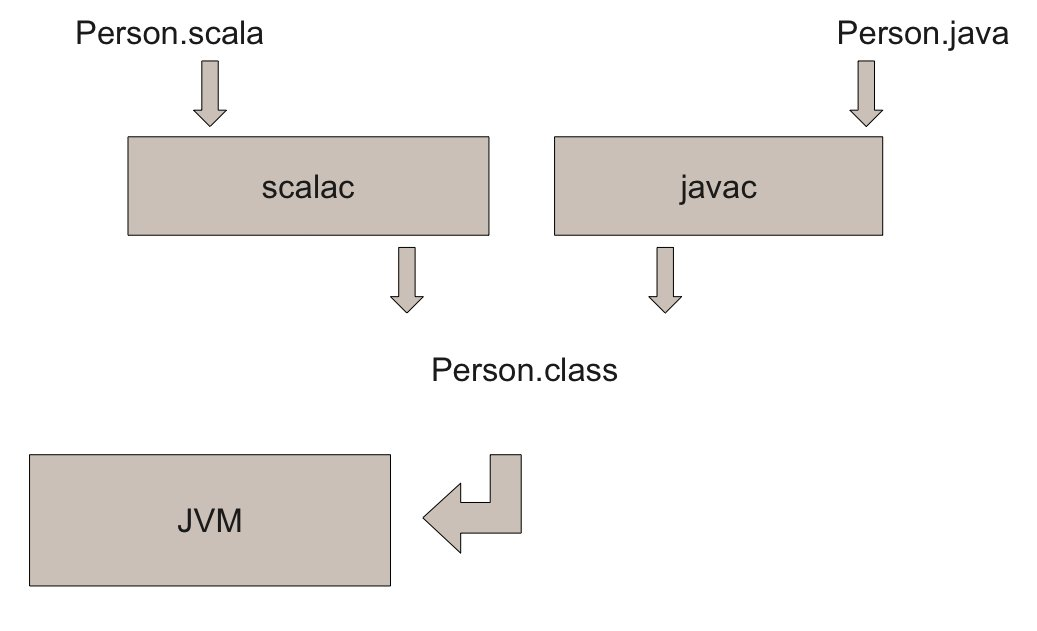
\includegraphics[height=17em]{jvm}
 \end {content}
\end{frame}

\begin{frame}[containsverbatim]{Helt grunnleggende -- Klasser}
 \begin{content}
\begin{lstlisting}[basicstyle={\small\ttfamily}]	   
class Person( //Konstrukt�rparametere og instansevariabler
   navn:String, 
   etternavn:String, 
   alder:Int)
{
  //Konstrukt�r
  val interesser = List("ting", "og", "tang") 
  val cv = "%s %s -- %s\n Liker: %s".format(
    navn, etternavn, alder, interesser.mkString(", ")
  )
  
  
  def fulltNavn ={ //Funksjon
    "%s %s".format(navn, etternavn) 
  }
}
     \end{lstlisting}
 \end {content}
\end{frame}

\begin{frame}[containsverbatim]{Helt grunnleggende -- val og var}
 \begin{content}
\begin{lstlisting}[basicstyle={\small\ttfamily}]	   

 //Er slik for altid
  val interesser = List("ting", "og", "tang") 
  
  def mineInteresser ={ 
    var interesser = "" //Kan tilordnes p� nytt
    for(interesse <- interesser){
    	interesser += interesse + ", "
    }
    
    interesser
  }
}
     \end{lstlisting}
 \end {content}
\end{frame}

\begin{frame}[containsverbatim]{Helt grunnleggende -- Oppgaver}
 \begin{content}
   Koden ligger her : https://github.com/aslakjo/scala\_intro\_kurs
   
   \begin{itemize}
     \item Last ned   
     \item G� til katalogen og kj�r 
     	\subitem{sbt}
     \item I sbt kj�r
     	\subitem{ update}
     	\subitem{\textasciitilde test-quick}
   \end{itemize}

 \end {content}
\end{frame}

\begin{frame}{Case classes}
  \begin{content}
  	En case classe er en normal klasse med masse ekstrautstyr 
  	\begin{itemize}
  		\item Genererer geters og seters
	  	\item Hash code og equals er implementert korrekt, og p� bakgrunn av verdiene
	  	\item Det companion object er laget
	  	\item Unapply / extractors er laget
	\end{itemize}
  	
  \end{content}
\end{frame}


\begin{frame}[containsverbatim]{Bruk av case classes}
  \begin{content}
    \begin{lstlisting}[basicstyle={\small\ttfamily}]	    	
	case class Sykkel(val farge:String, val hjul:Int) //def
	
	object CaseClassApp extends Application{
	  //compainon og new
	  assert(Sykkel("r�d", 2).equals(new Sykkel("r�d", 2))) 
	}
	
	//unapply kommer ..
    \end{lstlisting}
  \end {content}
\end{frame}

\begin{frame}{Patternmatching}
  \begin{content}
  	En veldig veldig kraftig variant av \it{switch} statementet 
  	\begin{itemize}
	  	\item Gir muligheten til � velge hele eller deler av et object
	  	\item Mulig � matche p� typer, verdier, arv, innhold i referanser
	\end{itemize}
  \end{content}
\end{frame}


\begin{frame}[containsverbatim]{Bruk av pattern matching}
  \begin{content}
    \begin{lstlisting}[basicstyle={\tiny\ttfamily}]	    			
	case class Farge(val navn:String)
	
	case class Bil(val farge:Farge, val hjul:Int)
	
	object PatternMatcingApp extends Application{
	  def godkjenntBil(dings: AnyRef)={
	    dings match {
	      //Constuctor pattarn, variabel pattern, med guard og extractor
	      case Bil(_, hjul) if hjul <= 2 => println("En slik bil heter gjerne motorsykkel")
	      //verdi pattern
	      case Bil(_, 4) => println("helt vanelig bil")
	      //sjekking i refererte objecter, variable pattern og guard
	      case Bil(Farge(fargePaBil), _) if fargePaBil.equals("r�d") => println("Jippi en r�d bil!")
	      //@ binder variabelen s til det som er p� h�yre side
	      case s@Bil(farve, _) if farve != null => println("dette er en " + farve.navn + " bil")
	      // type pattern
	      case s:Bil => println("dette er en bil")
	      //wildcard pattern, matcher alt
	      case _ => println("dette kan v�re hva som helst uten om en bil")
	    }
	  }
	}
    \end{lstlisting}
  \end {content}
\end{frame}

\begin{frame}{Traits}
  \begin{content}
	Et trait spesifiser egenskap.
  	\begin{itemize}
  		\item Kan brukes om interface(abstract traits)
		\item En klasse kan f� flere traits "mixet inn"  
		\item Traits kan ikke opprettes p� egenh�nd
	\end{itemize}
  \end{content}
\end{frame}

\begin{frame}[containsverbatim]{Bruk av traits}
  \begin{content}
    \begin{lstlisting}[basicstyle={\tiny\ttfamily}]
	trait HealthCheckable{ //interface
	  def isOk: Boolean
	}
	trait Logger { //egenskap
	  def log(message: String):Unit = println(message)
	}
	trait LoggProcessing extends FooService{ //stackable trait
	  def log(message:String):Unit
	
	  override def process:Unit={ //ny oppf�rsel
	    log("Starting processing")
	    super.process
	    log("Stopped processing")
	  }
	}
	
	class FooService extends HealthCheckable with Logger{ 
	  def isOk:Boolean = true
	
	  def process = {
	    //go allot!
	  }
	}
	
	object Application{  new FooService with LoggProcessing } //mix inn ved opprettelse
    \end{lstlisting}
  \end {content}
\end{frame}


\begin{frame}[plain]
  \begin{centering}
    
\includegraphics[height=11em]{bekk}
    \\\vspace{2em}\hfill\\
    \small
    
\includegraphics[height=1em]{bekk-logo}
    \\\vspace{.4em}\hfill\\
    \fontsize{8}{8}
    \selectfont
    \textbf{Aslak Johannessen}\\
    Senior Consultant\\
    982 19 249 \\
    aslakjo@bekk.no\\
    \vspace{.3em}\hfill\\
    \fontsize{1}{1}
    \selectfont
    BEKK CONSULTING AS\\
    SKUR 39, VIPPETANGEN. P.O. BOX 134 SENTRUM, 0102 OSLO, NORWAY. WWW.BEKK.NO\\
  \end{centering}
\end{frame}

\end{document}
